\chapter{New method for constrained non linear problems}
In general we are interested in nonlinear problems in which variables are constrained and, in particular, this is what happens in out test problem.  One of the ways to guarantee that the approximation of the solution respects the constraints, is to project the solution into the domain at each Newton's step, landing at the so-called projected Newton method.\\
 In this chapter we start introducing a new projected Newton-Krylov method for nonlinear problems, suggested in a recent paper called "Globalization technique for projected Newton-Krylov methods" published by Jinhai Chen and Cornelis Vuik \cite{MAIN}. The purpose is to fix the biggest defect of the already existing projected Newton-Krylov method, that is no guarantee of convergence, keeping all the advantages. Since, as we will see, the projected Newton direction is not always a descent one, while, if multiplied by a suitable scalar, the projected gradient direction it is , the idea is to switch on the second one all the times the fist one is not satisfactory.\\
 It was already known in theory that a sequence of $\{ \textbf{x}_k\} $, computed in this way $ \textbf{x}_{k+1} = \textbf{x}_{k} + \alpha \textbf{d}_k $, with $ \alpha $ a suitable length of the step and $ \textbf{d}_k $ a projected newton direction of $ \Theta (\textbf{x}_k) = \frac{1}{2} ||F (\textbf{x}_k)||^2$, converges to a stationary point of $ \Theta (\textbf{x}) $. What the authors of \cite{MAIN} add to the assertion, is that with a mixed use of projected Newton and projected gradient direction, $ \{\textbf{x}_k\} $ still ends in a stationary point, and more important, if the second direction is used finitely many times, then the sequences arrives in a zero of $ \Theta(\textbf{x}_k) $, which is what we are interested in.\\
 We report also two examples of the paper, one analytical, that shows a situation in which projected gradient direction is better that the projected newton one, and the other numerical, supposed to show the performance of the method. It was not easy to replay this one by ourselves, because lack of information, and in the end we realized that results shown in the paper were not compatible with the features of the concerned method, but at least we verified that, for that specific case, the use of projected gradient direction was essential, even if it was slow.\\
 All this analysis make us think that the strong point of this method is robustness rather then velocity.   

\section{Projected Newton-Krylov method}
The framework that we are going to consider is discretized system of nonlinear reaction diffusion equations in which the solutions has to be constrained in a certain interval.\\
A typical application was studied by van Veldhuizen, Vuik and Kleijn in \cite{before_MAIN}. They implemented the mathematical model of chemical vapor deposition, that is divided in three parts: Navier-Stokes equations, energy equations and advection-diffusion equations, that model the iterations of reactive species. The last part, discretized implicitly in time in order to guarantee stability, leads to a large-scale system of strongly nonlinear algebraic equations that need to be solved in each time step. Moreover, the variables are species mass fraction, so non-negativity is required for them, and the nonlinear system takes the following form.
\begin{equation*}
\begin{cases}
F(\textbf{x}) = 0\\ \textbf{x} \geq 0, 
\end{cases}
\end{equation*}
with $ F: \mathbb{R}^n \rightarrow \mathbb{R}^n  $ continuously differentiable and with around $10^9$ unknowns.
  The authors applied a \textit{projected Newton-Krylov method} to solve the system. What we mean with that name is defined in the Algorithm 1. \\
\begin{algorithm}
	\caption{projected Newton-Krylov}
	\label{pNK}
	\begin{algorithmic}[1]
		\STATE 	$ \textbf{x}_0 \in \mathbb{R}^{n}_{+} $, $ t \in (0,1) $, $ \eta_{max} \in [0,1) $, $ m_{max} \in \mathbb{N}  $ and $ 0 <  \lambda_{min} < \lambda_{max} < 1$
		\FOR{$k = 1, 2, \dots$ until convergence}
		\STATE Choose $\eta_k \in [0,\eta_{max}]$ and find $\textbf{d}_k$ that satisfy
		\STATE $ ||F(\textbf{x}_k) + F'(\textbf{x}_k)\textbf{d}_k||\leq \eta_k||F(\textbf{x}_k)|| $
		\STATE $ m = 0 $
		\WHILE { $m < m_{max}$}
		\STATE Choose $ \lambda \in  [\lambda_{min}, \lambda_{max}] $
		\IF{$ ||F(\mathcal{P}(\textbf{x}_k+ \lambda \textbf{d}_k))|| \leq (1 - t \lambda (1-\eta_k)) ||F(\textbf{x}_k)||$}
		\STATE	$ \textbf{x}_{k+1} = \mathcal{P}(\textbf{x}_k + \lambda \textbf{d}_k)$,  $m = m_{max} $
		\ELSE
		\STATE $ m = m + 1$
		\ENDIF
		\ENDWHILE
		\ENDFOR
	\end{algorithmic}
\end{algorithm}
In line 3 the forcing term $ \eta_k $ is computed with the techniques shown in section \ref{inexact_Newton_method} and in line 7 $ \lambda $ is chosen with line search methods, for example the ones illustrated in section \ref{line_search}. And, of course, as the name suggests, for the inexact Newton-method in line 4, it is used an iterative Newton-Krylov method for finding the solution $\textbf{d}_k $.
The other part of the name comes from the presence of $ \mathcal{P} $, that is a orthogonal projection on the domain, in this case $[0, \infty)$. So if we need non-negativity, we will have that the $i$th entry of $ \mathcal{P}(\textbf{x}) $ is defined by 
\begin{equation*}
\mathcal{P}_i(\textbf{x}) = \begin{cases}
x_i\;\;\;\; if\;\;\;\; x_i \geq 0\\ 0 \;\;\;\; \text{otherwise} .
\end{cases}
\end{equation*}
This is one of the simplest projection operator.
More precisely, this projection assigns to each component of $ \textbf{\textbf{x}} $, that is out of the constrains, the value of the broken restriction. So, in this case, non-negativity is prevent for all the variables of mass fraction.\\
An other important fact is that the local convergence of the Newton method is not affected, because of the non-expansiveness of the projection operator, as we will see in \textit{(c)} of Lemma \ref{lemma_grad}.

\section{Projected Newton-Krylov method mixed with projected gradient direction}
\subsection{Idea}
The work done in \cite{before_MAIN} shows that projected Newton-Krylov method is successful, where the classical nonlinear solver packages were not easy to use with such a big scale problem. Nevertheless, as the classical Newton method, this method does not guarantee global convergence; indeed, the search direction found by projected-Newton could not be a descent one, so could not minimize the norm of the underlying function $F$. Just to be more precise, defined $ \Theta (\textbf{x}) = \frac{1}{2} ||F(\textbf{x})||^2$, then $\textbf{d} $ is a descent direction for $\Theta (\textbf{x})  $ at point $\textbf{x}$ if  
\begin{equation}
\label{descentcond}
\frac{d \Theta (\textbf{x} + t\textbf{d})}{dt} |_{t=0} = \nabla \Theta (\textbf{x})^T \textbf{d} < 0 .
\end{equation}
Here comes the main idea of the numerical method that we have studied, taken from a recent paper "Globalization technique for projected Newton-Krylov methods" published by Jinhai Chen and Cornelis Vuik \cite{MAIN}. Knowing that a \textit{projected gradient direction} on a constrained set, that is $ \mathcal{P}(\textbf{x}_k - \lambda \nabla \Theta (\textbf{x}_k)) - \textbf{x}_k $, is \textit{usually} a descent one (Lemma \ref{lem_descent}), every time that the projected Newton-Krylov method is not able to find a descent direction, the algorithm will use a projected gradient one. 
The method that comes out still keeps the advantages of the projected Newton-Krylov method, as the capacity of solving extreme large-scale problems, the matrix-free operation, and preconditioning techniques, but it has also global convergence. The next step is to see how it happens. 

\subsection{Properties of the projector operator}
Before presenting in details this method, let us take a step back in a more general setting. Consider the following be a constrained system of nonlinear equations
\begin{equation*}
\begin{cases}
F(\textbf{x}) = 0\\\textbf{x} \in \Omega,
\end{cases}
\end{equation*}
where $\Omega$ is a convex constrained set of $\mathbb{R}^{n}$, such as $ \{\textbf{x} \in \mathbb{R} \; | \; \textbf{l} \leq \textbf{x}\leq \textbf{u}\}$, $l_i \in \{ \mathbb{R} \cup \{-\infty \}\} $ and $ u_i \in \{ \mathbb{R} \cup \{\infty\} \} $, $ l_i < u_i $ for all $ i = 1,...,n $, and $ F: \mathbb{R}^n \rightarrow \mathbb{R}^n  $ is continuously differentiable on $ \Omega $.

Let recall some properties of a projection operator. 
\begin{lem}{(see [\cite{Calamai}, Lemma 2.1])}
	\label{lemma_grad}
	Let $\varPi$ be the projection into $ \Theta  $.
	
	\begin{enumerate}[label=(\alph*)]
		\label{propertiesP}
		\item If $ \textbf{z} \in \Omega $ then $ (\varPi (\textbf{x}) - \textbf{x}, \textbf{z} - \varPi(\textbf{x}))\geq0 \; \; \forall \textbf{x} \in \mathbb{R}^n$ . 
		\item $ \varPi$ is a monotone operator, that is $(\varPi(\textbf{y}) - \varPi(\textbf{x}), \textbf{y} -\textbf{x})\geq 0  $ for $ \textbf{x}, \textbf{y} \in \mathbb{R}^n $. If $ \varPi(\textbf{y}) \neq\varPi(\textbf{x}) $, then strict inequality holds. 
		\item $ \varPi(\textbf{x}) $ is a non-expansive operator, that is, $||\varPi(\textbf{y}) - \varPi(\textbf{x})||\leq ||\textbf{y}-\textbf{x}|| $ for $ \textbf{x}, \textbf{y} \in \mathbb{R}^n$ 
	\end{enumerate}
\end{lem}
The next lemma is given by Gafni and Bertsekas in [\cite{Gafni}, Lemma 3] and [ \cite{Gafni2}, Lemma 1.a] and proven by Calamai and Mor\'e in [\cite{Calamai}, Lemma 2.2].
\begin{lem}
	\label{lem2paper}
	Let $ \varPi $ be a projection into $\Omega  $. Given $\textbf{x} \in \mathbb{R}^n $, then function $\psi  $ defined by 
	\begin{equation}
	\psi (\alpha) = \frac{||\varPi(\textbf{x} + \alpha d) - \textbf{x}||}{\alpha}, \; \alpha >0,
	\end{equation} 
	is antitone (non-increasing).
\end{lem}
With these properties, we arrive to say in the next lemma that the projected Newton-Krylov method, mixed with projected gradient direction, is well-defined, that is the projected gradient direction is descent.
\begin{lem}
	\label{lem_descent}
	Suppose that $ \textbf{x}_k $ is not a stationary point of $ \Theta(\textbf{x}_k) = \frac{1}{2}||F(\textbf{x}_k)||$ and $ \lambda \in (0,1] $. Then $ \mathcal{P}(\textbf{x}_k - \lambda \nabla \Theta (\textbf{x}_k)) - \textbf{x}_k $ is a descent direction for $ \Theta(\textbf{x}_k) $.
\end{lem}
\begin{proof}
	Let $ \textbf{x} = \textbf{x}_k - \lambda \nabla \Theta (\textbf{x}_k)$ and $ \textbf{z}= \textbf{x}_k $ in the part (a) of Lemma~\ref{propertiesP}. An immediate consequences of the part (a) of that lemma, says that 
	\begin{align*}
	0 & \leq \Bigl( \varPi \bigl(\textbf{x}_k - \lambda \nabla \Theta (\textbf{x}_k) \bigr) - \bigl(\textbf{x}_k - \lambda \nabla \Theta (\textbf{x}_k) \bigr), \textbf{x}_k - \varPi \bigl(\textbf{x}_k - \lambda \nabla \Theta (\textbf{x}_k)\bigr)\Bigr)\\
	& \leq \Bigl( \bigl(\varPi(\textbf{x}_k - \lambda \nabla \Theta (\textbf{x}_k)\bigr) - \textbf{x}_k , \textbf{x}_k-\varPi \bigl(\textbf{x}_k -  \lambda \nabla \Theta (\textbf{x}_k)\bigr) \Bigr) \\
	& \; \; \; \; + \Bigl( \lambda \nabla \Theta (\textbf{x}_k), \textbf{x}_k - \varPi \bigl(\textbf{x}_k - \lambda \nabla \Theta (\textbf{x}_k) \bigr)\Bigr)\\
	& \leq - ||\varPi \bigl(\textbf{x}_k - \lambda \nabla \Theta(\textbf{x}_k)\bigr) - \textbf{x}_k||^2 - \lambda \nabla \Theta(\textbf{x}_k)^T \bigl(\varPi(\textbf{x}_k - \lambda \nabla \Theta (\textbf{x}_k))-\textbf{x}_k\bigr).
	\end{align*}
	So we have for our particular projection $ \mathcal{P} $
	\begin{equation}
	\label{9P}
	\nabla\Theta (\textbf{x}_k)^T \bigl(\mathcal{P}(\textbf{x}_k - \lambda \nabla \Theta(\textbf{x}_k)) - \textbf{x}_k \bigr)\leq -\frac{1}{\lambda} ||\mathcal{P}(\textbf{x}_k -\lambda \nabla \Theta (\textbf{x}_k))- \textbf{x}_k||^2 < 0.
	\end{equation}
	This indicates that the projected gradient direction is descent for the norm of $ F(\textbf{x}_k) $.
\end{proof}

\subsection{Algorithm}
We report the expression of the new algorithm. \\

\begin{algorithm}[H]
	\caption{projected Newton-Krylov with projected gradient direction}
	\label{pNK}
	\begin{algorithmic}[1]
		\STATE 	$ \textbf{x}_0 \in \Omega $, $ t, \sigma \in (0,1) $, $ \eta_{max} \in [0,1) $, $ m_{max} \in \mathbb{N}  $, $ 0 <  \lambda_{min} \leq \lambda_0 \leq \lambda_{max} < 1$ and $ FLAG_{NG} = 0 $
		\FOR{$k = 1, 2, \dots$ until convergence}
				\IF {$ FLAG_{NG} = 0 $ and if a preconditioned Krylov subspace method finds some $ \eta_k \in [0, \eta_{max}] $ and a vector $ \textbf{d}_k $ satisfying
					\begin{equation}
					||F(\textbf{x}_k) + F'(\textbf{x}_k)\textbf{d}_k||\leq \eta_k||F(\textbf{x}_k)||
					\end{equation}
				}
    \algstore{testcont} 
	\end{algorithmic}
\end{algorithm}

\begin{algorithm}[H]
%	\caption{projected Newton-Krylov with projected gradient direction - Part 2}
	\begin{algorithmic}[1]
		\algrestore{testcont} 

		\STATE $ m = 0 $, $ \lambda = \lambda_{0} $ 
		\WHILE { $m < m_{max}$}
		\STATE Choose $ \lambda \in [\lambda_{min}, 1] $
		\IF{
			\begin{equation} 
			\label{ineqPN}
			||F(\mathcal{P}(\textbf{x}_k+ \lambda \textbf{d}_k))|| \leq (1 - t \lambda (1-\eta_k)) ||F(\textbf{x}_k)||
			\end{equation}
	     	}

		\STATE	$ \textbf{x}_{k+1} = \mathcal{P}(\textbf{x}_k + \lambda \textbf{d}_k)$,  $m = m_{max} $, $ FLAG_{NG}= 0 $
		\ELSE
		\STATE $ m = m + 1$, $FLAG_{NG} = 1 $
		\ENDIF
		\ENDWHILE
		\ELSE
		\STATE $ \textbf{d}_k = - \nabla \Theta (\textbf{x}_k) $
		\STATE $ m=0 $, $ \lambda = \lambda_0 $
		\WHILE { $m < m_{ma\textbf{x}}$}
		\STATE Choose $ \lambda \in  (0, 1]  $
		\IF{
			\begin{equation}
			\label{ineqPG} 
			\Theta(\mathcal{P}(\textbf{x}_k+ \lambda \textbf{d}_k)) \leq \Theta (\textbf{x}_k) + \sigma \nabla \Theta(\textbf{x}_k)^T (\mathcal{P}(\textbf{x}_k + \lambda \textbf{d}_k)- \textbf{x}_k)
			\end{equation}
		}
		\STATE	$ \textbf{x}_{k+1} = \mathcal{P}(\textbf{x}_k + \lambda \textbf{d}_k)$,  $m = m_{max} $, $ FLAG_{NG}= 0 $
		\ELSE
		\STATE $ m = m + 1$
		\ENDIF
		\ENDWHILE
		\ENDIF
		\ENDFOR
	\end{algorithmic}
\end{algorithm}
According to Lemma \ref{lem_descent}, the first part of \eqref{ineqPG}, that is $\Theta(\mathcal{P}(\textbf{x}_k+ \lambda \textbf{d}_k)) \leq \Theta (\textbf{x}_k)  $, should be always verified. Besides, the "task" of the second part, $ \sigma \nabla \Theta(\textbf{x}_k)^T (\mathcal{P}(\textbf{x}_k + \lambda \textbf{d}_k)- \textbf{x}_k) $, that is always negative, is to ensure that the new point makes the norm of $ F $ smaller "enough".

\subsection{Convergence results}
The authors Chen and Vuik display in \cite{MAIN} an interesting result for the convergence of this new method, that is the content of next theorem. 
\begin{theorem}
	\label{sppaper}
	Assume that $\{\textbf{x}_k\} \subset \Omega$ is a sequence generated by the feasible projected Newton-Krylov method. Then any accumulation point of $ \{\textbf{x}_k\} $ is at least a stationary point of $ \Theta(\textbf{x}_k) $. Further, if \eqref{ineqPN} is satisfied by the projected Newton direction for all but finitely many $ k $, then $\textbf{x}^*  $ is a zero of $ F(\textbf{x}) $ on $ \Omega $.
\end{theorem}
\begin{proof}
	Let $ \textbf{x}^* $ be an accumulation point of a sequence $ \{\textbf{x}_k\} $ generated by our method. The notation for $ \lambda $ that is used in the paper \cite{MAIN} is $ \lambda_0^{m_k} $, that indicates that  $ m_k $ is the power of $ \lambda_0 $, but to be more general, we can just say that $ \lambda_0^{m_k} $ is the $ \lambda $ picked up with an arbitrary technique at the $ m_k $th attempt in the line search loop for $ k $th nonlinear iteration. In addition, suppose that the first $\lambda  $ that we try for each nonlinear iteration $ k $ is $ \lambda_0^0 = 1 $. \\
	There are two cases.\\
	First, suppose that the projected Newton direction is used, so \eqref{ineqPN} holds, for finitely many iterations. It follows immediately that $ F(\textbf{x}^*) = 0$ because of the local convergence properties of the projected Newton method, that are the same of the classic one. So $ \textbf{x}^* $ is a stationary point.\\
	Second, suppose that the projected gradient direction is used (\eqref{ineqPG} holds) for all but finitely many iterations.
	It follows from \eqref{ineqPG} and from Lemma \ref{lemma_grad}, that $ \{\Theta (\textbf{x}_k)\} $ is monotonically decreasing (unless the method terminates at a stationary point at any finite step) and is bounded below by 0. Hence, it converges and 
	\begin{equation*}
	\lim_{k \rightarrow \infty} ( \Theta (\textbf{x}_{k+1}) - \Theta (\textbf{x}_k) ) = 0.
	\end{equation*}
	But then, using \eqref{ineqPG},we see that 
	\begin{equation}
	\label{lim11}
	\lim_{k \rightarrow \infty} \nabla \Theta (\textbf{x}_k)^T (\mathcal{P} (\textbf{x}_k - \lambda_0^{m_k} \nabla \Theta (\textbf{x}_k))- \textbf{x}_k)=0, 
	\end{equation}
	where $ \lambda_0^{m_k} $ can be seen as the lambda chosen at step $ k $.\\
	Let $ \{ \textbf{x}_k, k \in K \} $ be a subsequence converging to $\textbf{x}^*$. We have two cases for \eqref{lim11}.
	\textit{Case 1}: Assume 
	\begin{equation*}
	\liminf_{k (\in K) \rightarrow \infty}  \lambda_0^{m_k} > 0.
	\end{equation*}
	By \eqref{lim11} and  \eqref{9P}, it follows that for some infinite subset $ K' \subseteq K $,
	\begin{equation*}
	\lim_{k (\in K) \rightarrow \infty} - ||\mathcal{P}(\textbf{x}_k  - \lambda_0^{m_k} \nabla \Theta (\textbf{x}_k)) - \textbf{x}_k||^ 2= 0.
	\end{equation*}
	Hence, $ \textbf{x}^* $ is a stationary point of $ \Theta (\textbf{x}) $.\\
	\textit{Case 2}: Assume that there is a subsequence $ \{\textbf{x}_k\}_{k \in J}, J \subseteq K $ with 
	\begin{equation*}
	\lim_{k (\in J) \rightarrow \infty}  \lambda_0^{m_k} = 0.
	\end{equation*}
	So, for sufficiently large $k(\in J)$, $\textbf{x}_k$ is not a stationary point. Otherwise $ \lambda_0^{m_k} $ should be different from 0 because of \eqref{ineqPG}; in fact, if we have a stationary point, the first $ \lambda $ that we try should verify the inequality, that is $ \lambda_0^{m_k} = \lambda_0^0 = 1 $.\\
	Therefore, for sufficiently large $k(\in J) $, it holds that 
	\begin{equation}
	\label{14P}
	||\mathcal{P}(\textbf{x}_k - \lambda_0^{m_{k} -1} \nabla \Theta (\textbf{x}_k)) - \textbf{x}_k|| > 0,
	\end{equation} 
	because $ \textbf{x}_k $ is not a stationary point for all $ \lambda $ taken up to now, therefore also the previous one.  In addition, it follows from \eqref{ineqPG} that 
	\begin{equation*}
	\Theta(\mathcal{P}(\textbf{x}_k+ \lambda_0^{m_{k}-1} \textbf{d}_k)) - \Theta (\textbf{x}_k) > \sigma \nabla \Theta(\textbf{x}_k)^T (\mathcal{P}(\textbf{x}_k + \lambda_0^{m_{k}-1} \textbf{d}_k)- \textbf{x}_k).
	\end{equation*}
	Moreover, by the mean value theorem, we know 
	\begin{align*}
	\Theta(\mathcal{P} & (\textbf{x}_k - \lambda_0^{m_{k}-1} \nabla \Theta(\textbf{x}_k))) - \Theta (\textbf{x}_k) \\
	= & \nabla \Theta(\bm{\xi}_k)^T (\mathcal{P}(\textbf{x}_k - \lambda_0^{m_{k}-1} \nabla \Theta(\textbf{x}_k))- \textbf{x}_k)\\
	= & (\nabla \Theta(\bm{\xi}_k) - \nabla \Theta(\textbf{x}_k))^T (\mathcal{P}(\textbf{x}_k - \lambda_0^{m_{k}-1} \nabla \Theta(\textbf{x}_k))- \textbf{x}_k)\\
	& + \nabla \Theta(\textbf{x}_k)^T (\mathcal{P}(\textbf{x}_k - \lambda_0^{m_{k}-1}\nabla \Theta(\textbf{x}_k))- \textbf{x}_k) \\
	> &\sigma \nabla \Theta(\textbf{x}_k)^T (\mathcal{P}(\textbf{x}_k - \lambda_0^{m_{k}-1} \nabla \Theta(\textbf{x}_k))- \textbf{x}_k),
	\end{align*}
	where $ \bm{\xi}_k $ is a point in the line segment between $ \textbf{x}_k $ and $ \mathcal{P}  (\textbf{x}_k - \lambda_0^{m_{k}-1} \nabla \Theta(\textbf{x}_k)) $, so $ \bm{\xi} = \tau \textbf{x}_k + (1-\tau) \mathcal{P}(\textbf{x}_k - \lambda_0^{m_{k}-1} \nabla \Theta (\textbf{x}_k))$ for some $\tau \in (0,1)  $.
	Consequently, 
	\begin{align*}
	(\nabla \Theta(\bm{\xi}_k) - \nabla \Theta(\textbf{x}_k))^T & (\mathcal{P}(\textbf{x}_k - \lambda_0^{m_{k}-1} \nabla \Theta(\textbf{x}_k))- \textbf{x}_k)\\
	> &(1 -\sigma) \nabla \Theta(\textbf{x}_k)^T ( \textbf{x}_k - \mathcal{P}(\textbf{x}_k - \lambda_0^{m_{k}-1} \nabla \Theta(\textbf{x}_k))).
	\end{align*}
	Further, 
	\begin{equation} \label{18P}
	\begin{split}
	\nabla \Theta(\textbf{x}_k)^T & ( \textbf{x}_k - \mathcal{P}(\textbf{x}_k - \lambda_0^{m_{k}-1} \nabla \Theta(\textbf{x}_k)))\\
	< &\frac{1}{1 -\sigma} (\nabla \Theta(\bm{\xi}_k) - \nabla \Theta(\textbf{x}_k))^T(\mathcal{P}(\textbf{x}_k - \lambda_0^{m_{k}-1} \nabla \Theta(\textbf{x}_k))- \textbf{x}_k)\\
	< &\frac{1}{1 -\sigma} ||\nabla \Theta(\bm{\xi}_k) - \nabla \Theta(\textbf{x}_k)|| ||\mathcal{P}(\textbf{x}_k - \lambda_0^{m_{k}-1} \nabla \Theta(\textbf{x}_k))- \textbf{x}_k||.
	\end{split}
	\end{equation}
	From Lemma \ref{lem2paper}, we know that $ \frac{|| \textbf{x}_k - \varPi(\textbf{x}_k -  \lambda \nabla \Theta (\textbf{x}_k)) ||}{\lambda} $ is monotonically nonincreasing with respect to $ \lambda $. 
	From \eqref{9P}, we know that 
	\begin{align*}
	\nabla \Theta(\textbf{x}_k)^T & ( \textbf{x}_k - \mathcal{P}(\textbf{x}_k - \lambda_0^{m_{k}-1} \nabla \Theta(\textbf{x}_k)))\\
	\geq & \frac{|| \textbf{x}_k - \mathcal{P}(\textbf{x}_k -  \lambda_0^{m_k -1} \nabla \Theta (\textbf{x}_k)) ||^2}{\lambda_0^{m_k -1}}\\
	\geq & \frac{|| \textbf{x}_k - \mathcal{P}(\textbf{x}_k -  \lambda_0 \nabla \Theta (\textbf{x}_k)) ||}{\lambda_0} || \textbf{x}_k - \mathcal{P}(\textbf{x}_k -  \lambda_0^{m_k -1} \nabla \Theta (\textbf{x}_k)) ||,
	\end{align*}
	with the assumption that $ \lambda_0 \equiv \lambda_0^1 \geq \lambda_0^{m_k-1}$. \\
	This combined with \eqref{14P} and \eqref{18P}, implies 
	\begin{equation*}
	\frac{|| \textbf{x}_k - \mathcal{P}(\textbf{x}_k -  \lambda_0 \nabla \Theta (\textbf{x}_k)) ||}{\lambda_0} < \frac{1}{1-\sigma} ||\nabla \Theta (\bm \xi_k)  - \nabla \Theta (\textbf{x}_k)||.
	\end{equation*}
	Passing to the limit as $ k(\in J)\rightarrow \infty $, we obtain 
	\begin{equation*}
	\frac{|| \mathcal{P}(\textbf{x}_* -  \lambda_0 \nabla \Theta (\textbf{x}_*)) - \textbf{x}_* ||}{\lambda_0} = 0,
	\end{equation*}
	which implies $ \textbf{x}^* $ is a stationary point.  Therefore, in either case, we establish the assertion.
\end{proof}
The next result is about local convergence, but first we need to recall some concepts.\\ 
If $ F(\textbf{x}) $ is continuously differentiable, then $ F(\textbf{x}) $ is locally Lipshitz continuous at $ \textbf{x} $, that is, there exists a constant $ L_{\textbf{x}} $ such that for all $ \textbf{y} $
sufficiently close to $ \textbf{x} $, 
\begin{equation*}
||F(\textbf{y}) - F(\textbf{x}))|| \leq L_{\textbf{x}} ||\textbf{y} - \textbf{x}||.
\end{equation*}
Further, if $ F'(\textbf{x}) $ is nonsingular at $ \textbf{x}^* $, so there exists a constant $ C_{\textbf{x}^*} $ such that $ ||F'(\textbf{x}^*)^{-1}|| \leq C_{\textbf{x}^*} $, then there is a costant $ C $ such that $ F'(\textbf{y})^{-1} $ exists, and 
\begin{equation*}
||F'(\textbf{y})^{-1}|| \leq C
\end{equation*}
for all $ \textbf{y} $ sufficiently close to $ \textbf{x}^* $.
\begin{theorem}
	Assume that $\textbf{x}^* \in \Omega$ is a limit point of $\{\textbf{x}_k\} $ generated by the feasible projected Newton-Krylov method. Assume also that $F(\textbf{x}^*) = 0 $ and $F'(\textbf{x}^*)$ is nonsingular. Then the wole sequence $ \{\textbf{x}_k\}  $ converges to $ \textbf{x}^* $. Furthermore, for large enough $ k $, 
	
	\begin{enumerate}[label=(\alph*)]
		\item if $ \eta_{max} $ and $ t $ are chosen by 
		\begin{equation*}
		\begin{cases}
		\eta_{max} \in (0,1),\; \; t \in [C^2L, 1), \; \; \; if  \; \;C^2L < 1,\\
		\eta_{max} \in (0,\frac{1-t}{C^2L-t}),\; \; t \in (0, 1), \; \; \; if  \;	 \;C^2L \geq 1 	,
		\end{cases}
		\end{equation*}
		
		where $ L $ is the Lipschitz constant of $ F $ at $ \textbf{x}^* $ and $ C $ is an upper bound of inverse of $ F(\textbf{x}) $ defined in a neighborhood of $ \textbf{x}^* $, then the projected Newton direction is eventually accepted with $ \lambda = 1$, that is, no projection gradient is carried out.
		\item if 
		\begin{equation*}
		\begin{cases}
		\eta_{max} \in (0,\min\{ \frac{1}{CL}, 1\}),\; \; t \in [C^2L, 1), \; \; \; if  \; \;C^2L < 1,\\
		\eta_{max} \in (0,\min\{ \frac{1}{CL}, \frac{1-t}{C^2 L - t}\}),\; \; t \in (0, 1), \; \; \; if   \;C^2L \geq 1 	,
		\end{cases}
		\end{equation*}
		then the convergence rate is Q-linear;
		\item if $ \eta_k \rightarrow 0 $, the convergence rate is Q-superlinear.
	\end{enumerate}
\end{theorem}
\subsection{Previuos thoery of convergence for projected gradient direction}
Properties of projected gradient direction have been studied since 1960 and, in particular, we propose the handling of paper \cite{Calamai}. 
As we already know, gradient projection algorithm is defined by: 
\begin{equation}
\label{seqgrad}
\textbf{x}_k = P (\textbf{x}_k - \alpha_k \nabla \Theta(\textbf{x}_k)).
\end{equation}
In the convergence analysis of \cite{Calamai}, there is a theorem (Theorem 2.4) that states that if $\Theta : \mathbb{R}^n\rightarrow \mathbb{R}  $ is continuously differentiable on $ \Omega $, $ \{\textbf{x}_k\} $ be the sequence generated by \eqref{seqgrad}, with a suitable choice of $ \alpha_k $ and if some subsequence $ \{x_k, k \in K\} $ is bounded, then 
\begin{equation*}
\lim_{k \in K, k \rightarrow \infty} \frac{||\textbf{x}_{k+1} - \textbf{x}_k||}{\alpha_k} = 0
\end{equation*}
and any limit point of \eqref{seqgrad} is a stationary point of problem $\Theta(\textbf{x})$.
This result means it was already known that if we use only projected gradient direction, the sequence of $ \textbf{x}_k $ is going to converge in a stationary point. Theorem \ref{sppaper} adds that the mix of projected Newton directions and projected gradient directions ends still in a stationary point, moreover, if the second ones are used finitely many times, it reachs a point in which $ \Theta(\textbf{x}) = 0 $, that, actually, is our concern. \\
In general the projected gradient of $ \Theta(\textbf{x}) $ is defined by 
\begin{equation}
\nabla_{\Omega} \Theta( \textbf{x} ) \equiv argmin \{ || v + \nabla  \Theta ( \textbf{x} ) || : v \in T( \textbf{x} ) \},
\end{equation} 
where $T(\textbf{x}) $ is the \textit{tangent cone}, closure of the cone of feasible directions. In our case $ \nabla_{\Omega} \Theta (\textbf{x}_k) =  P(\textbf{x}_k - \nabla \Theta(\textbf{x}_k)) - \textbf{x}_k $. It is shown that this operator has the following properties. 
\begin{lem}
	Let $ \nabla_{\Omega} \Theta (\textbf{x}) $ be the projected gradient of $ \Theta $ at $ \textbf{x} \in \Omega$.
	\begin{enumerate}[label=(\alph*)]
		\item $ -(\nabla \Theta (\textbf{x}),\nabla_{\Omega} \Theta (\textbf{x})  )= ||\nabla_{\Omega} \Theta (\textbf{x})||^2 $.
		\item $ \min \{(\nabla \Theta (\textbf{x}),v) : v \in T(\textbf{x}), ||v|| \leq 1 \} = - || \nabla_{\Omega} \Theta (\textbf{x})||$.
		\item The point $ \textbf{x} \in \Omega $ is a stationary point of $ \Theta(\textbf{x}) $ if and only if $ \nabla_{\Omega} \Theta(\textbf{x}) = 0 $.
	\end{enumerate}
\end{lem}
Point $ (b) $ is important because it is displays that $ \nabla_{\Omega} \Theta (\textbf{x}) $ is a steepest descent direction for $ \Theta $, so we can say that our projected gradient direction $  P(\textbf{x}_k - \nabla \Theta(\textbf{x}_k)) - \textbf{x}_k  $ is still the steepest one in $ \Omega $.
\subsection{Examples}
\subsubsection{Analytical example}
We report one simple example that shows how projected gradient direction can "save" situations in which the projected Newton direction cannot be descent. 
Consider the following constrained problem for $ \textbf{x} = (x_1, x_2)^T \in \Omega = (-\infty, 1] \times (-\infty, 1] $:
\begin{equation*}
\begin{cases}
x_1^2 - x_2 -2 = 0,\\
x_1 - x_2 = 0,
\end{cases}
\end{equation*}
with $\textbf{x}^* = (-1,-1)^T  $ unique solution in $ \Omega $. We have :
\begin{eqnarray*}
	F'(\textbf{x}) = \begin{pmatrix}
		2x_1 & -1 \\
		1 & -1
	\end{pmatrix}&,\\
	\nabla \Theta (\textbf{x}) = (2x_1(x_1^2-x_2-2)+x_1-x_2,& -(x_1^2-x_2-2)-(x_1-x_2))^T.
\end{eqnarray*}
If we take $ \textbf{x}_0 = (1, \frac{1}{2})^T $, then it follows that the Newton direction is $ \textbf{d}_0 = (2, \frac{5}{2})^T $ with $ \eta_0 = 0 $ in Algorithm \ref{pNK}. As we know from theory, this direction, if calculated exactly, is a descent one; indeed:
\begin{equation*}
\nabla \Theta (\textbf{x}_0)^T\textbf{d}_0 = \left(-\frac{5}{2}, 1\right) \cdot \left(2, \frac{5}{2}\right)^T = - \frac{5}{2} < 0.
\end{equation*}
The problem comes when we project it because we find
\begin{eqnarray*}
	P (\textbf{x}_0 +\lambda \textbf{d}_0) - \textbf{x}_0 &= \left( \min\{1+2\lambda, 1 \},\min \{1, \frac{1}{2} + \frac{5\lambda}{2}\} \right)^T - \left(1, \frac{1}{2}\right)^T \\
	&=\left(0, \min \{\frac{1}{2}, \frac{5\lambda}{2} \}\right),
\end{eqnarray*}
and therefore
\begin{eqnarray*}
	\nabla \Theta (\textbf{x}_0)^T (P (\textbf{x}_0 +\lambda \textbf{d}_0) - \textbf{x}_0) &= \left(-\frac{5}{2}, 1\right) \cdot \left(0, \min \{\frac{1}{2}, \frac{5\lambda}{2}\}\right)^T\\
	&= \min\{ \frac{1}{2}, \frac{5 \lambda}{2} \} \geq 0,
\end{eqnarray*}
for any $ \lambda \in (0,1] $. We conclude that in this case the projected Newton direction can not be descent, but, as we expect from Lemma \ref{lem_descent}, the projected gradient direction has to be a good one; indeed:
\begin{eqnarray*}
	P (\textbf{x}_0 -\lambda \nabla \Theta (\textbf{x}_0)) - \textbf{x}_0 &= \left( \min\{1+\frac{5}{2}\lambda, 1 \},\min \{1, \frac{1}{2} - \lambda\} \right)^T - \left(1, \frac{1}{2}\right)^T \\
	&=\left(0,-\lambda \right)^T,
\end{eqnarray*}
and
\begin{equation*}
\nabla \Theta (\textbf{x}_0)^T (P (\textbf{x}_0 -\lambda \nabla \Theta (\textbf{x}_0)) - \textbf{x}_0) = \left(-\frac{5}{2}, 1\right) \cdot \left(0,-\lambda \right)^T = - \lambda < 0.
\end{equation*}
The geometrical scenario is illustrated in Figure \ref{esempio7}, where we see that the projected Newton direction (PND) cannot be descent, because it lies on the semi-plane in which the function is supposed to grow, and that the projected gradient (PGD) is still descent. 
\begin{figure}[h]
	\centering
	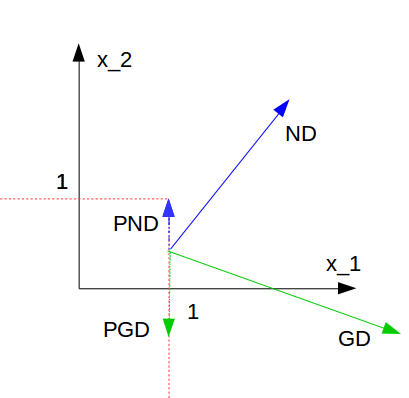
\includegraphics[width=0.7\linewidth]{example7}
	\caption[Newton and gradient direction]{Blue arrows are Newton directions (projected and not), while green ones are gradient directions (projected and not). We see how the projected Newton direction (PND) is increasing for the norm of $ F $ since it lies in the semi-plane in which the function is supposed to grow, that is the semi-plane that has the opposite of the GD. Instead, the projection of the gradient direction (PGD) is in the decreasing semi-plane.}
	\label{esempio7}
\end{figure}

\subsubsection{Numerical example}
In addiction to the analytical example that we have just shown, there is also a numerical one in \cite{MAIN} (Example 8), whose aim is to show the performances of the new projected Newton-Krylov method. It is about a system of nonlinear equations for $ \textbf{x} = (x_1, \dots, x_n)^T $ with $ \Omega = \{ \textbf{x} \in \mathbb{R}^n | x_1 \in [0.8, 2], x_i \in [0.5, 2], 2 \leq i \leq n \} $. The system is
\begin{equation*}
\begin{cases}
x_1^2 - 1 = 0,\\
x_1 - x_2^3 = 0,\\
x_2 - x_3^3 = 0, \\
\; \;  \; \; \vdots \\
x_{n-2} - x_{n-1}^2 = 0,\\ 
x_{n-1} - x_n = 0
\end{cases}
\end{equation*}
with solution  $ \textbf{x}^* = (1, \dots, 1)^T $ in $ \Omega $.\\ 
As a first approach, we tried to implement this problem by our self with $ n = 100 $ in order to compare our results with the ones of the paper. The information that we had about settings of Algorithm \ref{pNK}, was the following: 
\begin{enumerate}[label=(\alph*)]
	\item initial guess for the nonlinear iterations $ \textbf{x}_0 (1:20) = 0.9  $ and $ \textbf{x}_0 (21:100) = 0.5$, and zero vector for the linear ones;
	\item termination tolerance rule for nonlinear iteration: $ ||F(\textbf{x}_k)|| \leq 10^{-12} $;
	\item choice of linear search parameter $ \lambda = \lambda_0^ m$, with $ \lambda_0 = 0.5 $ for porjected Newton direction and $ \lambda_0 = 0.8 $ for projected gradient one.
	\item $ \sigma = t = 10^{-4} $, $ m_{max} = 20 $, $ \eta_{max} = 0.9 $;
	\item linear solver GMRES.
\end{enumerate}
For the choice of forcing term $ \eta_k $ the authors just say that they used one of the options in \cite{Forcingterm}, the ones that we illustrated in the previous chapter. The problem for us was that we did not know exactly which one was the choice used and which was the value of the parameters. Using all information we had and the values of residual norm $ ||F(\textbf{x})|| $ that we should have obtained (table in Figure \ref{results_example8}), we applied a reverse iterative technique to find out the forcing terms. In practice, we interpolated the tolerance needed in the linear solver (so the forcing term) to arrive to the residual norms of Figure \ref{results_example8} and, after few steps, we found that they used Choice 2 \eqref{Choice2} with $ \alpha = 2 $, $ \gamma = 0.9 $ and $ \eta_0 \simeq 0.765518 $.\\
\begin{figure}[h]
	\centering
	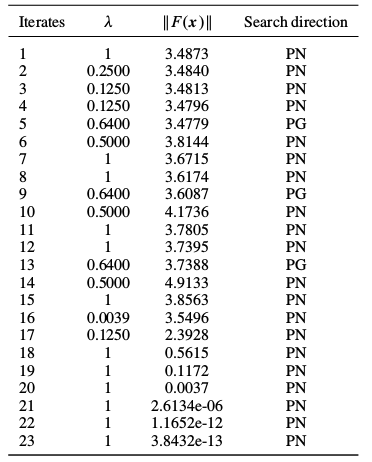
\includegraphics[width=0.6\linewidth]{results_example8}
	\caption[Table of results of example 8 in \cite{MAIN}]{Table of results of Example 8 in \cite{MAIN}, PN indicates that it was used projected Newton direction and PG projected gradient direction. The values of columns of $ \lambda $ and $ ||F(\textbf{x})|| $ are shifted by one respect to the others; indeed the norm of $ F $ that was achieved in iteration 1 and the $ \lambda $ that was used are the one in the second row.}
	\label{results_example8}
\end{figure}
First of all, we have to point out that in Figure \ref{results_example8}, each value of $ ||F(\textbf{x})|| $ is actually the input value of that iteration, so, for example, $ 3.4873 $ corresponds to $ ||F(\textbf{x}_0)|| $, and the value in the second iteration is the residual norm that comes from the first iteration. The same is true for values of $ \lambda $ , so the columns of $ \lambda $ and $ ||F(\textbf{x})|| $ are shifted by one iteration respect to the other two columns.\\
After all this procedure, we realized that the values of $ \lambda $ in iterate 5 and 6 are reported wrongly, indeed in 5, $ \lambda $ is equal actually to $ 0.5^2 $ and not to $ 0.8^2 $ because it refers to the previous step that uses PN, and not PG. Indeed in 6, $ \lambda$ is equal to $0.8 $ and not to $ 0.5 $ for the same reason. This correction needs to be done for iterates 9, 10, 13 and 14 as well. We have reported our results in Figure \ref{our_example8} in the same format as in Figure \ref{res_paper}.\\
Another thing that we noticed, more important, was that, in order to have the same results as in the paper's Table, we had to force $ \lambda $ to be equal to $ 0.8 $ in each time PG was used, even if \eqref{ineqPG} was not verified. When we did the test as Algorithm \ref{pNK} indicates, at iteration 5, $ \lambda = 0.8 $ was not enough, so the algorithm selected $ \lambda = 0.8^4 $ to satisfy \eqref{ineqPG}. Therefore, all the convergence behavior, that follows step 5, changes. Figure \ref{res_paper} and \ref{res_our}, shown their and our trend of the residual norm.\\
\begin{figure}[h]
	\centering
	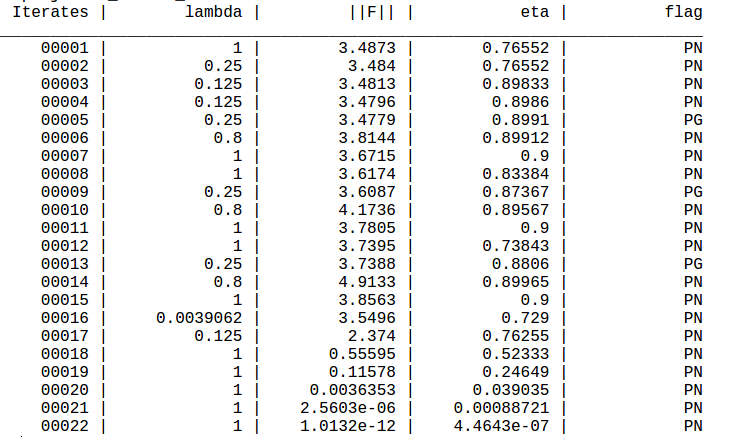
\includegraphics[width=1\linewidth]{ourresults8}
	\caption[Table of our results for example 8 in \cite{MAIN}]{Table of our results for Example 8 in \cite{MAIN}. We manage to generate this results, that are equal to the ones in Figure \ref{results_example8}, at least in the first 16 iterations, with a revers iterative technique that found the missed information, that is the choice for $ \eta_k $. But we had also to impose $ \lambda = 0.8 $ in each PG step, even if the inequality \eqref{ineqPG} was not satisfied.}
	\label{our_example8}
\end{figure}
\begin{figure}[h]
	\centering
	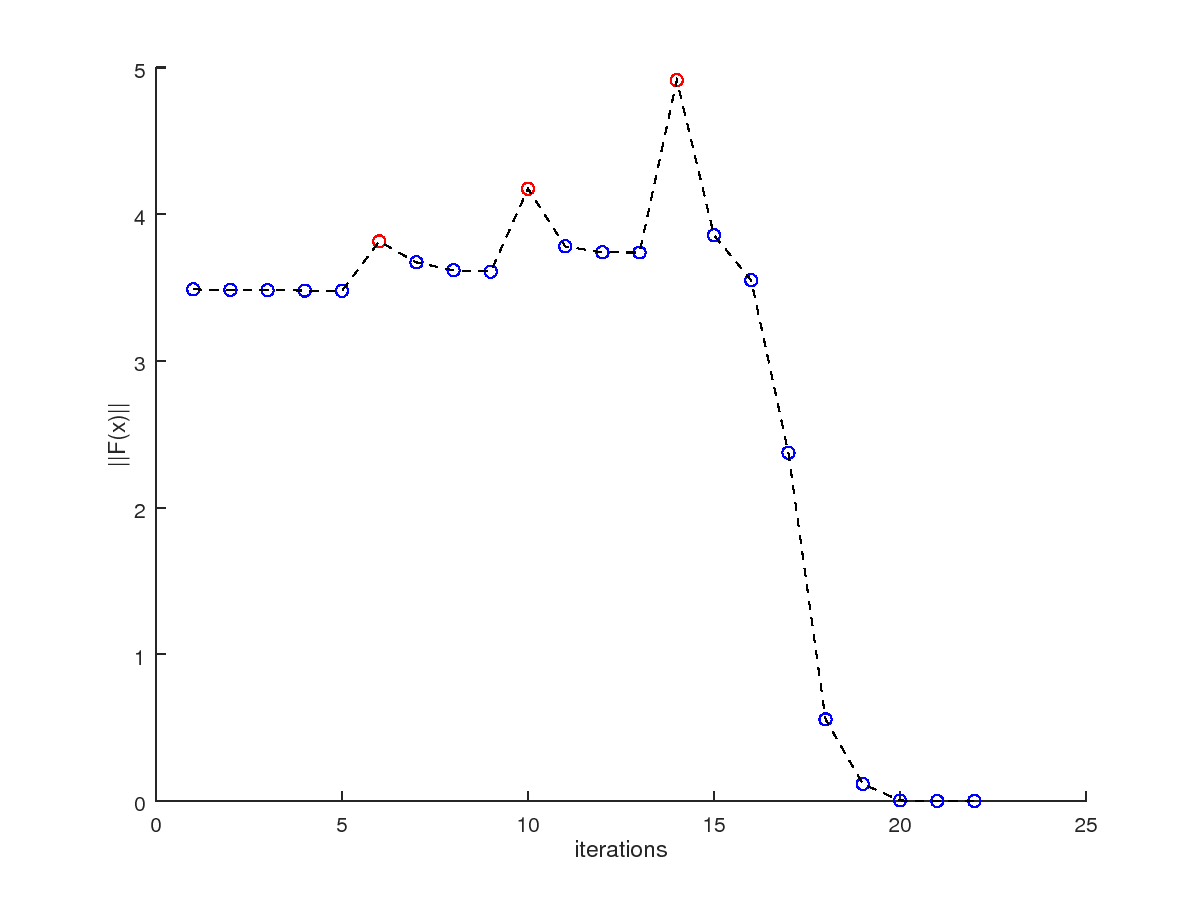
\includegraphics[width=0.8\linewidth]{res_paper}
	\caption[Plot of residuals found in \cite{MAIN}]{Residual norms according to paper's result, blu point are PN and red ones are PG. We see that they does not respect the main characteristic of the analyzed method, that is that the norm of $ F $ has not to increase. This happens because inequality \eqref{ineqPG} is not satisfied.}
	\label{res_paper}
\end{figure}
\begin{figure}[h]
	\centering
	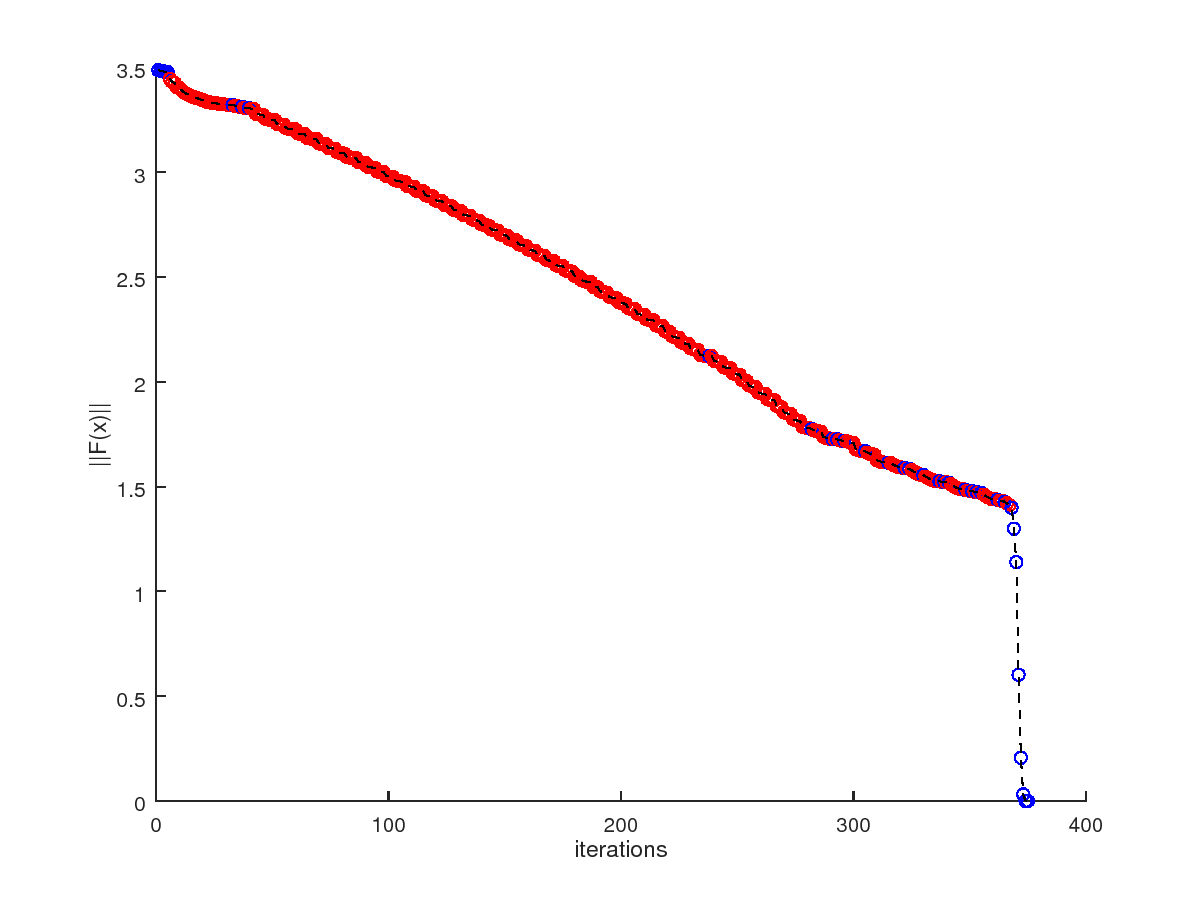
\includegraphics[width=0.8\linewidth]{res_our}
	\caption[Plot of residuals found by us]{Residual norms that we obtained implementing Algorithm \ref{pNK} in the right ways. In this case the number of iterations is much bigger than the one promised in the paper and a lot of PG are used, reason for which the convergence is slow.}
	\label{res_our}
\end{figure}
Actually, there was no need to implement all by our self to see that there is something wrong. In fact, if we notice the trend of the residual norm in Figure \ref{results_example8} and \ref{res_paper}, we realize that is not non-increasing. That should not happen when \eqref{ineqPG} is verified, since $ \sigma $ has to be positive and $\nabla \Theta(\textbf{x}_k)^T (\mathcal{P}(\textbf{x}_k + \lambda \textbf{d}_k)- \textbf{x}_k)  $ has to be negative because the projected gradient direction is a descent one (Lemma \ref{lem_descent}). So the residual norm has to be strictly decreasing. \\
We have discovered that in our implementation much more iterations were required to reach convergence and for most of them it is used projected gradient direction, so the decrease of residual norm is very slow. Indeed the use of PG cannot be considered as a massive one because it is too slow, it should intervene in isolated steps when PN is not able to find a acceptable direction. \\
In any case, we tried to implement the algorithm without PG and we verified that it is not going to converge because the PN forces $\textbf{x} $ to arrive to the other solution $ \textbf{x}^* = (-1, \dots, -1)^T$, that is out of $ \Omega $, so $ \textbf{x} + \lambda \textbf{d} $ is always projected on the constraints, consequently the algorithm remains stuck. 
